\chapter{Tổng quan}
\label{Chapter1}

\section{Tổng quan về trí tuệ nhân tạo}
\subsection{Trí tuệ nhân tạo}
\subsubsection*{Khái niệm}
Con người đã, đang và sẽ mãi mãi khao khát phát minh ra những thứ giúp cuộc sống của họ dễ dàng hơn và tốt đẹp hơn gấp ngàn lần. 
Khả năng mà tâm trí con người có thể làm luôn khiến chúng ta bối rối. Một trong những phát minh quan trọng như vậy sẽ là thứ được gọi 
là AI- Trí tuệ nhân tạo . Sẽ không tuyệt sao nếu máy móc có thể suy nghĩ? Đó chính xác là AI. Con người chúng ta có trí thông minh tự nhiên. 
Nhưng nếu máy móc có thể suy nghĩ, nó sẽ là nhân tạo. Vì vậy, AI chỉ là một thuật ngữ chung cho những cỗ máy có thể suy nghĩ. Kể từ khi được 
đề xuất vào năm 1950, AI đã phát triển vô cùng mạnh mẽ, đặc biệt là những năm gần đây. Một số lĩnh vực con của AI đã ra đời đó là học máy và nhỏ
hơn nữa là học sâu. 

% insert image
\begin{figure}[h]
\centering
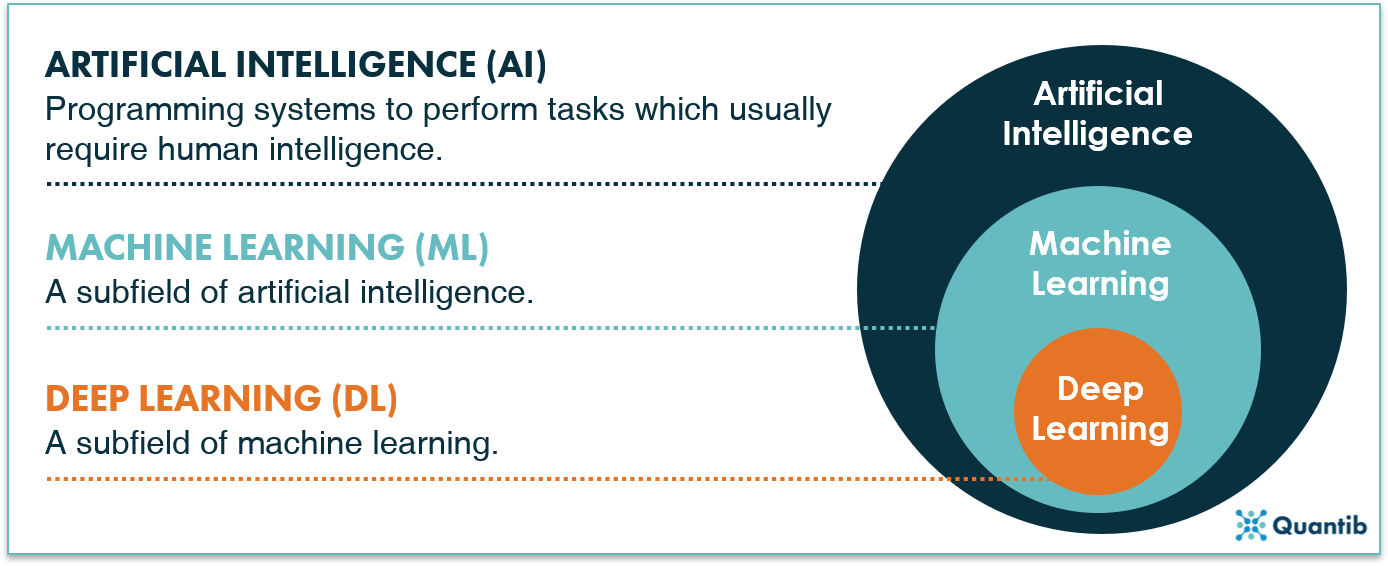
\includegraphics[width=\textwidth]{Image/AI.png}
\caption{AI}
\label{Hình 1.1: AI}
\end{figure}

\subsubsection*{Ứng dụng của AI trong đời sống}
\begin{itemize}
    \item Y tế:
    
        AI được sử dụng khá phổ biến trong lĩnh vực y tế như chuẩn đoán hình ảnh X quang, phát hiện các loại bệnh trên người.
    
    \item Kinh tế:
    
        AI được sử dụng rất nhiều trong công nghiệp như robot, các dây chuyền tự động. Đặc biệt với khả năng thu thập cũng như phân tích dữ liệu, trí tuệ AI có thể
        nắm bắt thông tin cũng như hành vi sử dụng dịch vụ của khách hàng, từ đó mang lại những giải pháp hữu ích trong kinh doanh, đây là một trong những ứng dụng được sử
        dụng nhiều nhất của các công ty công nghệ lớn như Facebook hay Amazon.
    \item Giáo dục:
    
        AI có thể được sử dụng vào các hoạt động như chấm điểm, hay giám sát thi cử của học sinh, sinh viên.

\end{itemize}


\subsection{Học máy}
\subsubsection*{Khái niệm}
Học máy là lĩnh vực nghiên cứu cung cấp cho máy tính khả năng học hỏi mà không cần lập trình rõ ràng. ML là một trong những công nghệ thú vị nhất mà người ta từng thấy. Như rõ 
ràng ngay từ cái tên, nó khiến cho máy tính giống với con người hơn \textbf{"Khả năng học hỏi".}
Học máy được chia làm hai loại chính là học có giám sát và học không giám sát.

\subsubsection*{Học có giám sát}
Học có giám sát , còn được gọi là học máy có giám sát, được xác định bằng cách sử dụng các bộ dữ liệu được gắn nhãn để huấn luyện các thuật toán nhằm phân loại dữ liệu hoặc dự đoán kết 
quả một cách chính xác. Khi dữ liệu đầu vào được đưa vào mô hình, mô hình sẽ điều chỉnh trọng số của nó cho đến khi nó được điều chỉnh phù hợp. Điều này xảy ra như một phần của quy trình 
xác thực chéo để đảm bảo rằng mô hình tránh bị thừa  hoặc  thiếu . Học có giám sát giúp các tổ chức giải quyết nhiều vấn đề trong thế giới thực ở quy mô lớn, chẳng hạn như phân loại 
thư rác trong một thư mục riêng biệt với hộp thư đến. Một số phương pháp được sử dụng trong học có giám sát bao gồm neural networks, linear regression, logistic regression, 
random forest, và support vector machine (SVM).  

\subsubsection*{Học không giám sát}
Học không giám sát , còn được gọi là học máy không giám sát, sử dụng các thuật toán học máy để phân tích và phân cụm các bộ dữ liệu không được gắn nhãn. Các thuật toán này khám phá các mẫu 
hoặc nhóm dữ liệu ẩn mà không cần sự can thiệp của con người. Khả năng khám phá những điểm tương đồng và khác biệt trong thông tin của phương pháp này khiến nó trở nên lý tưởng cho việc phân 
tích dữ liệu khám phá, chiến lược bán chéo, phân khúc khách hàng cũng như nhận dạng hình ảnh và mẫu. Nó cũng được sử dụng để giảm số lượng các tính năng trong một mô hình thông qua quá trình 
giảm kích thước. Phân tích thành phần chính (PCA) và phân tích giá trị đơn lẻ (SVD) là hai cách tiếp cận phổ biến cho việc này. Các thuật toán khác được sử dụng trong học tập không giám sát bao 
gồm mạng thần kinh, phương pháp phân cụm k-means hoặc k-means++.

\subsection{Học sâu}
\subsubsection*{Khái niệm}
Học sâu là một tập hợp con của  học máy , về cơ bản là một mạng thần kinh có ba lớp trở lên.
Mạng thần kinh học sâu, hay mạng thần kinh nhân tạo, cố gắng bắt chước bộ não con người thông qua sự kết hợp của dữ liệu đầu vào, trọng số và độ lệch. Các yếu tố này hoạt động cùng nhau để nhận dạng, 
phân loại và mô tả chính xác các đối tượng trong dữ liệu.

\subsubsection*{Cách thức hoạt động}
Mạng lưới thần kinh sâu bao gồm nhiều lớp nút được kết nối với nhau, mỗi lớp được xây dựng dựa trên lớp trước đó để tinh chỉnh và tối ưu hóa dự đoán hoặc phân loại. Quá trình tính toán này thông qua 
mạng được gọi là lan truyền thuận. Các lớp đầu vào và đầu ra của mạng nơ-ron sâu được gọi là  các lớp hiển thị  . Lớp đầu vào là nơi mô hình học sâu nhập dữ liệu để xử lý và lớp đầu ra là nơi đưa ra dự đoán hoặc phân loại cuối cùng.

Một quy trình khác được gọi là lan truyền ngược  sử dụng các thuật toán, chẳng hạn như giảm độ dốc, để tính toán lỗi trong các dự đoán, sau đó điều chỉnh trọng số và độ lệch của hàm bằng cách di chuyển ngược qua các lớp nhằm nỗ lực 
huấn luyện mô hình. Cùng với nhau, lan truyền xuôi và lan truyền ngược cho phép mạng nơ-ron đưa ra dự đoán và sửa bất kỳ lỗi nào tương ứng. Theo thời gian, thuật toán dần trở nên chính xác hơn.

\section{Tổng quan về TensorFlow}

\subsection{TensorFlow là gì?}
Với sự bùng nổ của lĩnh vực Trí Tuệ Nhân Tạo – A.I. trong thập kỷ vừa qua, machine learning và deep learning rõ ràng cũng phát triển theo cùng. 
Và ở thời điểm hiện tại, TensorFlow chính là thư viện mã nguồn mở cho machine learning nổi tiếng nhất thế giới, được phát triển bởi các nhà nghiên 
cứu từ Google. Việc hỗ trợ mạnh mẽ các phép toán học để tính toán trong machine learning và deep learning đã giúp việc tiếp cận các bài toán trở 
nên đơn giản, nhanh chóng và tiện lợi hơn nhiều. 

Hiện nay, TensorFlow cơ bản được xem như một trong những phương tiện trung gian giúp tính toán cho các số lượng có trong sản xuất và đồng thời trở 
thành một công cụ không thể thiếu trong Machine Learning, cùng với sự tương thích với nhiều ngôn ngữ lập trình như C++, Python, Java... 
Từ đó, phục vụ cho nhu cầu học tập cũng như nghiên cứu một cách dễ dàng hơn. 

Tensor được hiểu là một loại cấu trúc dữ liệu được tập hợp 
trong một thư viện mà ở đó chính là TensorFlow. Trong số đó, cấu trúc của dữ liệu sẽ được miêu tả rồi điều chỉnh theo nhiều cách sao cho phù hợp 
nhất với các kiểu dữ liệu này. Và, cấu trúc dữ liệu này sẽ bao gồm 3 thuộc tính chính là: Bậc, chiều và loại dữ liệu. 


Các hàm được dựng sẵn trong thư viện cho từng bài toán cho phép TensorFlow xây dựng được nhiều neural network. 
Nó còn cho phép tính toán song song trên nhiều máy tính khác nhau, thậm chí trên nhiều CPU, GPU trong cùng 1 máy hay tạo ra các dataflow graph – đồ 
thị luồng dữ liệu để dựng nên các model.






\subsection{Cách TensorFlow hoạt động}
Kiến trúc của Tensorflow cơ bản bao gồm 3 phần chính là: 
\begin{itemize}
\item \textbf{Tiền xử lý dữ liệu}
\item \textbf{Dựng Model}
\item  \textbf{Train và ước tính Model}
\end{itemize}

Khi TensorFlow hoạt động sẽ cho phép các lập trình viên có thể tạo ra dataflow graph, cũng như cấu trúc mô tả làm sao để cho dữ liệu có thể di chuyển 
qua 1 biểu đồ; hoặc di chuyển qua 1 seri mà các node đang xử lý. Mỗi một node có trong đồ thị thường đại diện cho 1 operation toán hoặc và mỗi kết nối 
thường hay edge giữa các node với nhau.

Từ đó, mỗi kết nối hoặc edge giữa các node được xem là mảng dữ liệu đa chiều. TensorFlow sẽ cung cấp tất cả mọi điều đến cho lập trình viên dựa theo 
phương thức của ngôn ngữ Python. Ngôn ngữ này sẽ cung cấp nhiều cách tiện lợi để ta có thể hiểu được nên làm thế nào cho các high-level abstractions 
có thể kết hợp được với nhau. Node cũng như tensor có trong TensorFlow chính là đối tượng của Python. Và, mọi ứng dụng Tensorflow bản thân chúng chính 
là một ứng dụng Python. 

Các operation toán học thực sự thì thường không được thi hành bằng Python. Những thư viện biến đổi thường không có sẵn thông qua TensorFlow được viết 
bằng các binary C++ có hiệu suất cao.
Ngoài ra, Python chỉ điều hướng cho các lưu lượng giữa các phần cũng như cung cấp các high-level abstraction lập trình để có thể nối chúng lại với nhau. 
Train thường phân tán dễ chạy hơn nhờ vào API mới và sự hỗ trợ cho TensorFlow Lite để cho phép việc triển khai các mô hình trên với nhiều nền tảng khác nhau. 

\subsection{Adam Optimizer}
Adam là viết tắt của Adaptive Moment Estimation là một thuật toán cho kỹ thuật tối ưu hóa để giảm dần độ dốc. Adam có hiệu quả cao và được sử dụng rộng rãi 
trong các bài toán học máy. Phương pháp này thực sự hiệu quả khi làm việc với bài toán lớn liên quan đến nhiều dữ liệu hoặc tham số. Nó đòi hỏi ít bộ nhớ hơn và hiệu quả. 
Nó là sự kết hợp của thuật toán "gradient descent" và "RMSProp".

\subsubsection*{Gradient descent with momentum}
Thuật toán gradient descent with momentum được sử dụng để tăng tốc thuật toán giảm độ dốc bằng cách xem xét "trung bình trọng số theo cấp số nhân" của độ dốc. 
Sử dụng mức trung bình làm cho thuật toán hội tụ về phía cực tiểu với tốc độ nhanh hơn.

\begin{equation}
\begin{aligned}
m_t & = \beta_1 m_{t-1} + (1 - \beta_1) \frac{\delta L}{\delta w_t} \\
w_t & = w_{t-1} - \alpha m_t\\
\end{aligned}
\end{equation}

trong đó :

\begin{itemize}
\item $m_t$ là tổng các gradient tại thời điểm t. (với $m_0 = 0$)
\item $v_t$ là tổng các gradient tại thời điểm t-1.
\item $\beta$ là tham số trung bình.
\item $\alpha$ là tốc độ học.
\item $\delta L$ là đạo hàm của hàm mất mát.
\item $w_t$ là trọng số tại thời điểm t.
\item $w_{t-1}$ là trọng số tại thời điểm t-1.  
\end{itemize}

\subsubsection*{Root Mean Square Propagation (RMSP)}
Root mean square prop hay RMSprop là một thuật toán học thích ứng cố gắng cải thiện AdaGrad. Thay vì lấy tổng tích lũy của bình phương độ dốc như trong AdaGrad, 
nó lấy "trung bình động hàm mũ".

\begin{equation}
\begin{aligned}
v_t & = \beta v_{t-1} + (1 - \beta) (\frac{\delta L}{\delta w_t})^2 \\
w_t & = w_{t-1} - \alpha_t \frac{\delta L}{\delta w_t} \frac{1}{\sqrt{v_t + \epsilon}}\\
\end{aligned}
\end{equation}

trong đó:

\begin{itemize}
\item $v_t$ tổng bình phương của gradient trong quá khứ.
\item $\beta$ là tham số trung bình.
\item $\alpha$ là tốc độ học.
\item $\delta L$ là đạo hàm của hàm mất mát.
\item $w_t$ là trọng số tại thời điểm t.
\item $w_{t-1}$ là trọng số tại thời điểm t-1.
\item $\epsilon$ là một hằng số dương rất nhỏ để tránh chia cho 0.
\item $\delta w_t$ là đạo hàm của trọng số tại thời điểm t .

\end{itemize}

\textbf{Adam Optimizer} kế thừa các điểm mạnh hoặc thuộc tính tích cực của hai phương pháp trên và dựa trên chúng để tạo ra độ dốc giảm dần được tối ưu hóa hơn.

\subsection*{Công thức toán học của Adam Optimizer}
Từ 2 công thức 1.1 và 1.2 ta có :
\begin{equation}
\begin{aligned}
m_t & = \beta_1 m_{t-1} + (1 - \beta_1) \frac{\delta L}{\delta w_t} \\
v_t & = \beta_2 v_{t-1} + (1 - \beta_2) (\frac{\delta L}{\delta w_t})^2 \\
\hat{m_t} & = \frac{m_t}{1 - \beta_1^t} \hat{v_t} \\
w_t & = w_{t-1} - \alpha_t \frac{\hat{m_t}}{\sqrt{\hat{v_t}} + \epsilon}\\
\end{aligned}
\end{equation}

trong đó:

\begin{itemize}
\item $\beta_1$ và $\beta_2$ tốc độ phân rã trung bình của các gradient trong hai phương pháp trên.
\item $\hat{m_t}$ và $\hat{v_t}$ là các tham số trọng số đã hiệu chỉnh sai lệch.
\end {itemize} 
Từ đó ta thu được:
\begin{equation}
    \begin{aligned}  
    w_t & = w_{t-1} - \alpha_t \frac{\hat{m_t}}{\sqrt{\hat{v_t}} + \epsilon}\\
\end{aligned}
\end{equation}

Dựa trên những điểm mạnh của các mô hình trước đó, trình tối ưu hóa Adam mang lại hiệu suất cao hơn nhiều so với mô hình được sử dụng trước đây và vượt trội hơn
chúng một cách đáng kể trong việc tạo ra độ dốc giảm dần được tối ưu hóa. Biểu đồ được hiển thị bên dưới mô tả rõ ràng cách trình tối ưu hóa của Adam vượt trội 
so với phần còn lại của trình tối ưu hóa bằng một biên độ đáng kể về chi phí đào tạo (thấp) và hiệu suất (cao). 

\begin{figure}[h!]
    \centering
    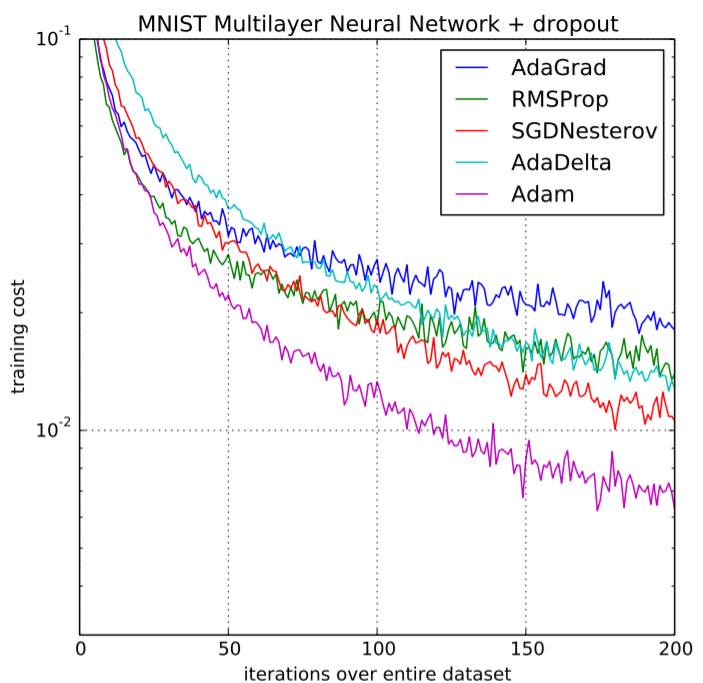
\includegraphics[width=0.8\linewidth]{Image/Adam.png}
    \caption{So sánh các thuật toán tối ưu hóa}
    \label{Hình 1.1: Graph Neural Network}
    \cite*{WEBSITE:3}
\end{figure}


\textbf{Trong TensorFlow} thuật toán tối ưu hóa Adam được sử dụng với các thông số mặc định của các công thức trên là $\alpha$ = 0.001, $\beta_1$ = 0.9, $\beta_2$ = 0.999, và $\epsilon$ = 1e-8. 
Các thông số này có thể dễ dàng tùy biến bằng cách gán các giá trị cho các thuộc tính tương ứng có sẵn trong Adam.

